\documentclass[ngerman,12pt]{scrreprt}

\usepackage{babel}
\usepackage{blindtext}
\usepackage{microtype}
\usepackage{graphicx}
\usepackage{amsmath}
\usepackage{esvect}
\usepackage{siunitx}








\author{\textbf{drayvila}}
\title{Miene Dissertation}

\usepackage{hyperref}
\hypersetup{
    bookmarks=true,                     % show bookmarks bar
    unicode=false,                      % non - Latin characters in Acrobat’s bookmarks
    pdftoolbar=true,                        % show Acrobat’s toolbar
    pdfmenubar=true,                        % show Acrobat’s menu
    pdffitwindow=false,                 % window fit to page when opened
    pdfstartview={FitH},                    % fits the width of the page to the window
    pdftitle={My title},                        % title
    pdfauthor={Author},                 % author
    pdfsubject={Subject},                   % subject of the document
    pdfcreator={Creator},                   % creator of the document
    pdfproducer={Producer},             % producer of the document
    pdfkeywords={keyword1, key2, key3},   % list of keywords
    pdfnewwindow=true,                  % links in new window
    colorlinks=true,                        % false: boxed links; true: colored links
    linkcolor=blue,                          % color of internal links
    filecolor=blue,                     % color of file links
    citecolor=blue,                     % color of file links
    urlcolor=blue                        % color of external links
}


\begin{document}

\maketitle

\tableofcontents

\listoftables

\listoffigures



\chapter{Einführung}

\blindtext




\begin{figure} [b]
\begin{center}
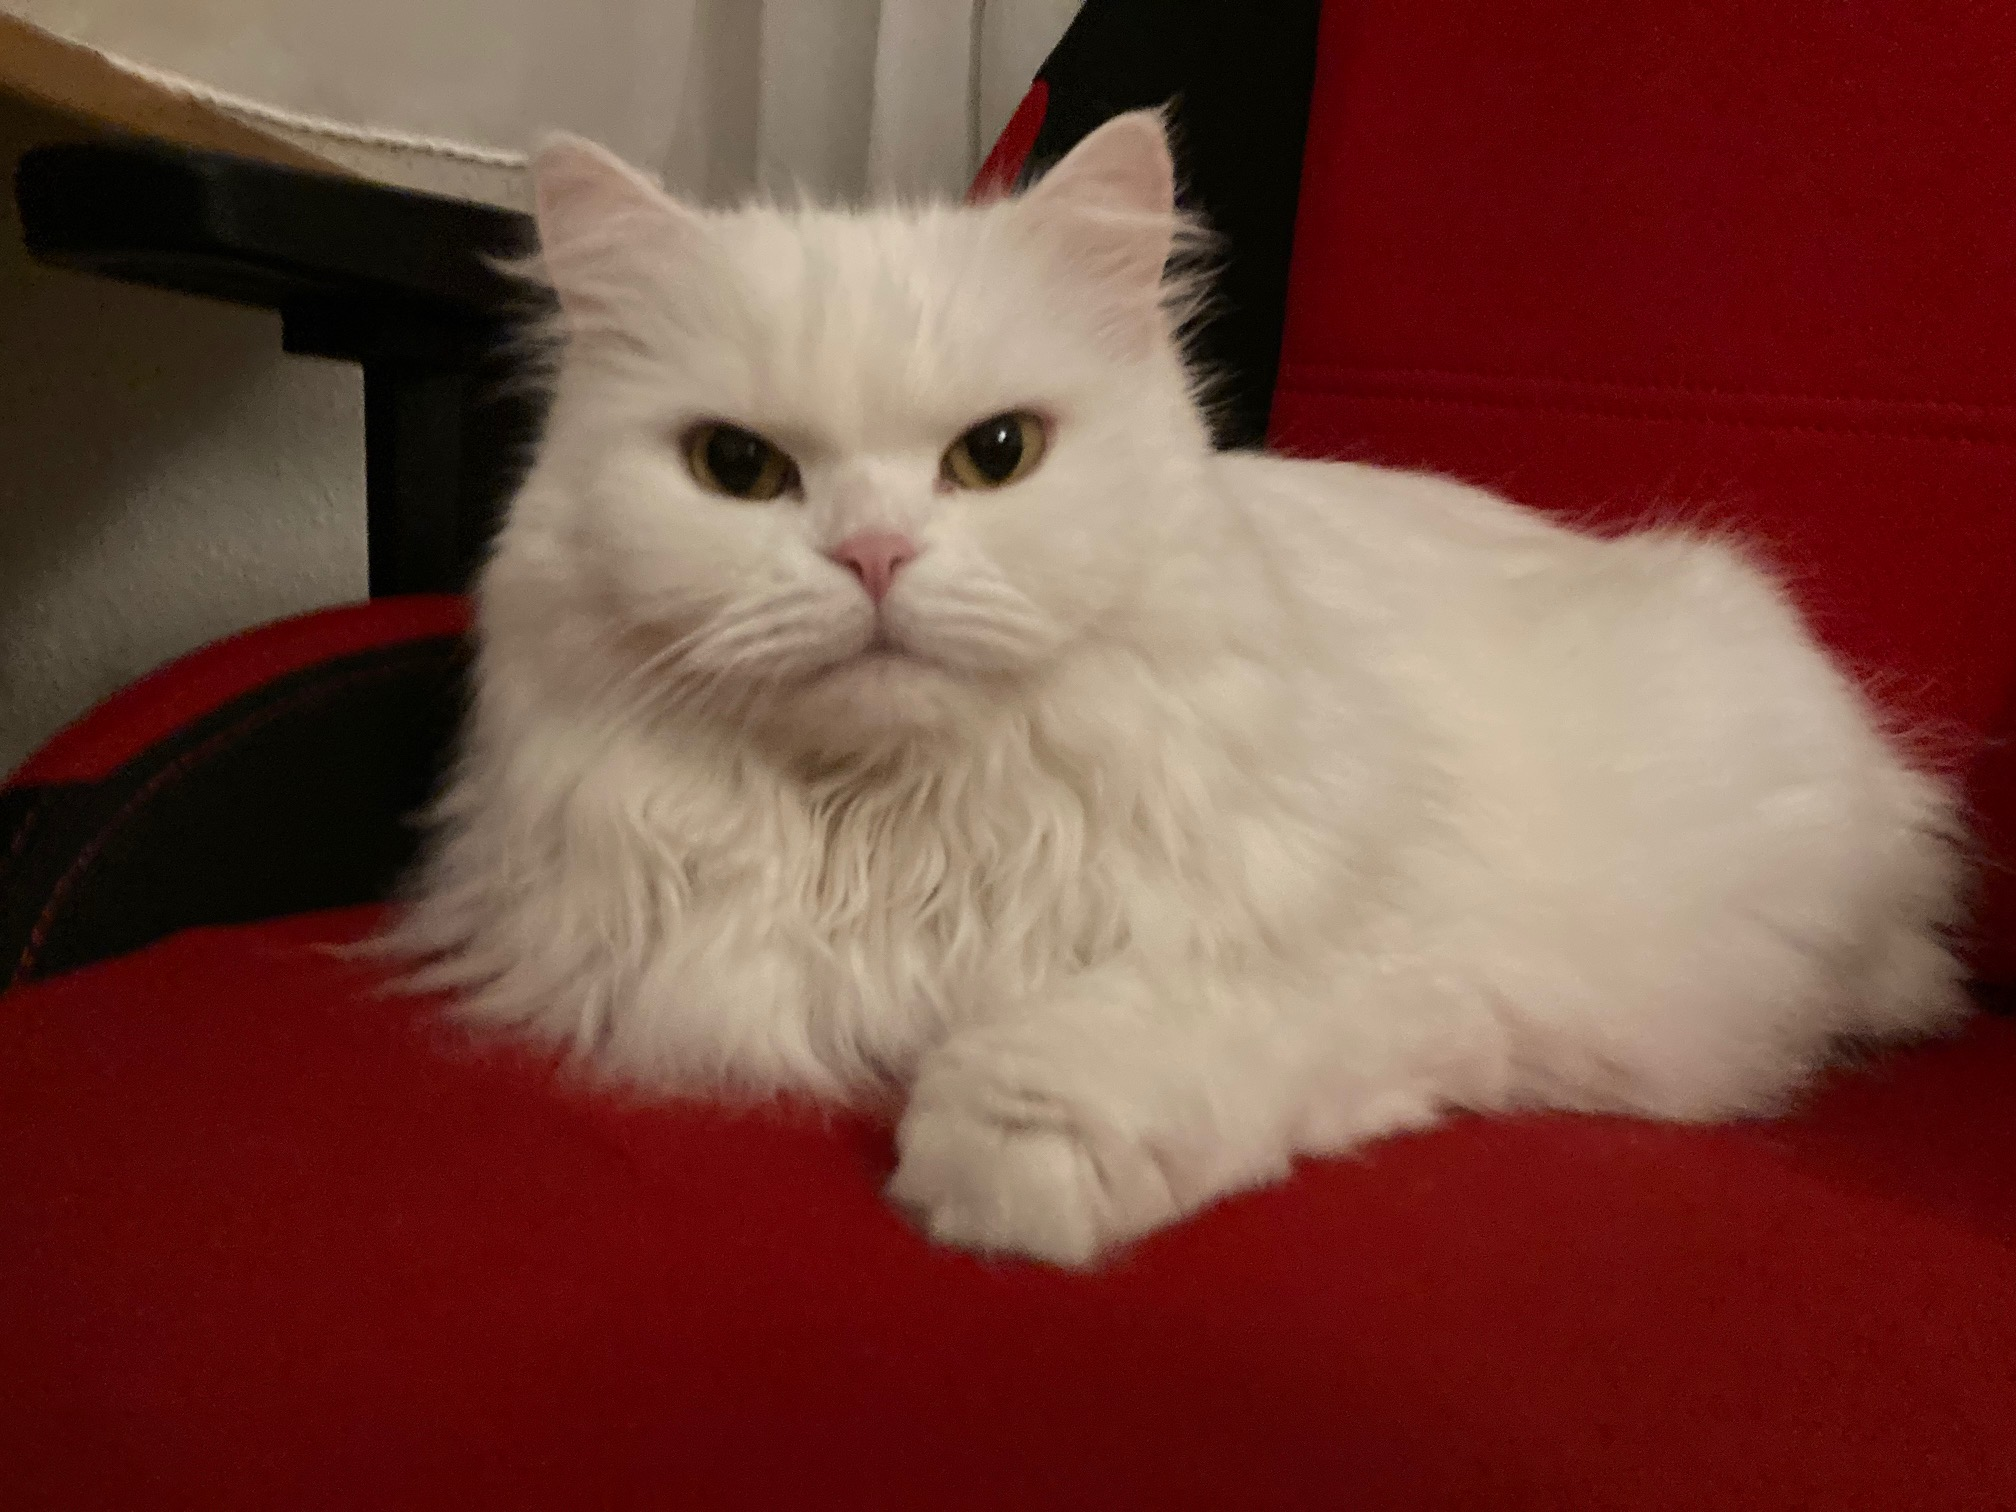
\includegraphics[width=5cm]{Katze2}
\caption{unsere Miezekatze}\label{fig:katze}
\end{center}
\end{figure}

\chapter{Mathematik}
TeX-Notaion im Fließtext $a^2 + b^2 = c^2$


\[a^2 + b^2 = c^2\] \\

Siehe equation \ref{eq:sinnlos} in page \pageref{eq:sinnlos}


\[
\bordermatrix{%
  & 0 & 1 & 2 & 3\cr
 0 & A & B & C & D\cr
 1 & A & B & C & D\cr
 2 & A & B & C & D\cr
}
\]



\section{AMS Beispiele}

\begin{equation} \label{eq:sinnlos}
\begin{pmatrix}
A & B & C \\
A & B & C \\
A & B & C \\
\end{pmatrix}
\end{equation}

\begin{equation}
\begin{bmatrix}
A & B & C \\
A & B & C \\
A & B & C \\
\end{bmatrix}
\end{equation}

\begin{equation}
\begin{Bmatrix}
A & B & C \\
A & B & C \\
A & B & C \\
\end{Bmatrix}
\end{equation}

\begin{equation}
z = \beta 
\begin{vmatrix}
A & B & C \\
A & B & C \\
A & B & C \\
\end{vmatrix}
\end{equation}

\begin{equation}
\sum_{i=1}^{\infty^2} i^3
\end{equation}


 \[
 \gamma
 \]

% esvect Paket für den \\vv{ Befehl}
\[ \vv{a} \cdot \vv{abc} \]


a\quad b c

% AMS MATH

\begin{align}
a &= x \cdot y
\end{align}


\section*{Nicht ijm Anhaltverzeichniss}
\begin{align*}
a &= x \cdot y
\end{align*}

\begin{alignat}{3}
a &= bbb &&= t \cdot y \\
aaa &= b &&= \sin x \cdot \cos y \\
a &= 44 \\
u &= u_{4}^4
\end{alignat}

\chapter{Einheitensatz mit siunitx}

1cm \\

\num{3,1456478} oder \num{54545464}

\si{m} \si{m\per \second^2} $1m^2$

\SI{4570008}{\kilo\meter\per\second}

\SIrange{10}{20}{\kilo\meter\per\second}

\ang{180}


\vspace*{2cm}
\begin{tabular}{rS}
a & 123.456 \\
a & 123.45675675656 \\
a & 123454554.456 \\
a & 123.456 \\
a & 123.456e10 \\
a & 123.456 \\
\end{tabular}

\end{document}









